\chapter{Quantum Computing: A brief overview}
\label{chap:Overview}

\section{The principles of quantum computing}
\label{Principles}

The advantages of using quantum mechanics to perform computations come down to the following three principles:

\begin{itemize}

\item \textit{Superposition}: In classical computing, the unit of information is the \textit{bit}, which may take one of two values: \(0\) or \(1\). In quantum computing, the \textit{bit}'s counterpart is the \textit{qubit}, whose value may be \textit{any linear combination} of the \(0\) state and the \(1\) state, known as a \textit{superposition}, and usually written as: \[\ket{qubit} = \alpha\ket{0} + \beta\ket{1}\] where \(\alpha\) and \(\beta\) are complex numbers that must satisfy: \(\alpha^2 + \beta^2 = 1\).

A popular analogy of a qubit's superposition is a coin spinning\footnote{Note this is just an analogy, and while a coin spinning can be perfectly described using classical physics, a qubit can not.}: the classical states (\(0\) and \(1\)) are \textit{heads} and \textit{tails}, but when the coin is spinning, its state is neither of them. If we knew exactly how the coin was spinning, we would be able to describe the probability of seeing heads or tails when it stops; these would be our \(\alpha^2\) and \(\beta^2\) values. Besides, we may \textit{measure} a qubit, and doing so corresponds in our analogy to abruptly stopping the coin, then checking if it is \textit{heads} or \textit{tails}. Through certain operations -- that would correspond to altering the axis of spin of the coin --, we may change the coefficients \(\alpha\) and \(\beta\) of the superposition. 

In most quantum programs, we encode input and read output (after measurement) as standard classical binary strings. Therefore, for input/output we use as many qubits as bits would be required. Superposition allows us to maintain -- during mid-computation -- a superposition of all potential solutions to the problem, and update all of them simultaneously with a single operation to the qubits. In some sense, superposition allows us to explore multiple choices/paths of the computation, using only the resources required to explore a single one of those paths. And the number of paths we can explore simultaneously can be up to exponential, as a collection of \(N\) qubits may be in a state of superposition of all the possible \(2^N\) classical states.

\item \textit{Interference}: As we just discussed, superposition gives us the ability to simultaneously explore different paths to solve a problem. However, in the end we will need to measure the qubits -- stop the coins -- and the result will be intrinsically random. For quantum computing to be any better than a probabilistic classical computer, we require the ability to prune the paths that have led to a result we do not want. This is precisely what \textit{interference} provides: some operations on the qubits may make different classical states in the superposition cancel each other out. Interference is at the core of any speed-up achieved by a quantum algorithm, and taking advantage of it is the main challenge when designing quantum algorithms.

\item \textit{Entanglement}: Quantum mechanics allows the possibility of having a pair of qubits \(a\) and \(b\) in a superposition such as: \[\ket{a,b} = \frac{1}{\sqrt{2}}\ket{0,0} + \frac{1}{\sqrt{2}}\ket{1,1}\] This implies that, when we measure the qubits, we may either read \(a=0, b=0\) or \(a=1, b=1\) as outcome, never \(a\not=b\) (the coefficients for \(\ket{0,1}\) and \(\ket{1,0}\) are both \(0\)). Then, what happens if we only measure \(a\)? In this particular case, we would also know \(b\)'s outcome, without measuring it. In short, acting on one qubit has an instantaneous effect on the other. Whenever a group of qubits exhibits this property, we say they are \textit{entangled}. Entanglement holds regardless how far apart \(a\) is from \(b\); for instance, they could be on two different quantum processing units of a distributed grid. Indeed, entanglement will be key in our discussion of distributed quantum algorithms, and we explain how to use it to perform non-local operations in \S\ref{IntroDistributing}.

\end{itemize}


\section{Building quantum computers}
\label{Hardware}

Physicists have come up with different ways of realising qubits in labs. The key idea is to find a physical system that displays non-classical behaviour, and put it under the appropriate circumstances so we can manage its quantum properties. At the same time, we must ensure that noise from the environment does not interfere with our quantum information. \citet{ArchitectureSurvey} give an excellent survey of the state of the art of quantum architectures. Among these, the three most developed are:

\begin{itemize}

\item \textit{Quantum optics}: The state of a qubit is represented in the properties of photons, for instance, their polarisation~\citep{OpticsQC}. A great advantage of this technology is that photons can be easily sent over long distances, while preserving their quantum state. Thus, protocols in quantum information that heavily rely on communication, such as Quantum Key Distribution~\citep{QKD}, are usually discussed and experimented with using quantum optics. The downside of this technology is that it is very difficult to make photons interact, which is required for universal computation.

\item \textit{Ion-traps}: Each qubit is embodied as an ion, confined inside a chamber by means of an electric or magnetic fields. The qubit is acted upon by hitting the ion with electromagnetic pulses (e.g.\ laser light or microwave radiation). Groups of experimentalists have proposed how to scale up the technology~\citep{HensingerIonTraps}, and are currently building prototypes.

\item \textit{Superconductors}: Small circuits, similar to classical electrical circuits, are cooled down to near absolute zero so the quantum interactions of electrons are not obscured by other perturbations. Different parts of the circuit encode different qubits, which can be acted upon by applying electric potentials. One of the main advantages of this approach is that the technology required for building the chips is fairly similar to the one for classical computer chips. This technology is the most experimentally developed. In fact, using it, both IBM and Intel have already built small generic-purpose quantum computers with up to 50 qubits, and Google claims to own a 72 qubit machine.

\end{itemize}

However, for quantum computers to be useful in real world applications, their qubit count should be larger than that. And, unfortunately, increasing the amount of qubits in a quantum computer is particularly difficult, due to some challenges we will now discuss.


\subsection{Scalability challenges}
\label{Challenges}

There are two main challenges to overcome in order to build large scale quantum computers:

\begin{itemize}

\item \textit{Decoherence}: In \S\ref{Principles} we discussed the importance of having superposition in quantum computing, and we compared a qubit in superposition with a coin spinning. For similar reasons why a coin spinning will eventually stop, a qubit in superposition will eventually degenerate into a classical state (i.e.\ either \(\ket{0}\) or \(\ket{1}\)). This phenomenon is known as \textit{decoherence}. Experimentalists attempt to increase the time it takes for the state of the qubit to degenerate\footnote{A fundamentally different approach, \textit{anyonic} (a.k.a.\ topological) quantum computing, has been proposed to avoid the problem of decoherence altogether. It would use physical systems that, theoretically, can be completely protected against decoherence~\citep{Anyonic}. Although promising, currently this proposal has little experimental underpinning, and it is not regarded as attainable in the near future.}. Decoherence is the main constraint to scalability for quantum computers, as it limits the lifespan of qubits, limiting the number of operations that can be applied in a single program. 

Certainly, the state of bits also degenerates in classical computers. However, in their case this is easier to account for: we can monitor the bits, and make sure to correct any unwanted change. This is not so simple in quantum computers, as monitoring a qubit would require \textit{measuring} it, which destroys any quantum superposition. Nevertheless, it is still to some extent possible to protect our quantum state from errors -- either due to decoherence or imperfect hardware -- through specialised quantum error correction routines~\citep{QuantumErrorCorrection}. This is a very active area of research, and it will be essential for the implementation of reliable large scale quantum computers.


\item \textit{Connectivity}: In order to run any computation on qubits, we will need to be able to apply multi-qubit operations on any subset of the computer's qubits. However, it is not realistic to expect that quantum computers will have fast connectivity between all qubits, for instance due to spatial separation of these in the hardware. In classical systems, the same problem is solved by a memory hierarchy, with a ceaseless flow of data going up and down of it, from main memory to registers (where computation is performed) and back. The memory hierarchy model works because data can stay idly in main memory while computation on the registers is carried out. However, in quantum computers we must avoid qubits being idle, as decoherence prevents the existence of long-lasting memory. An alternative found in classical computers is to distribute the computation across different processing units each having its own local memory, which they use intensively. In these distributed systems, communication across computers is the main bottleneck, and it should be performed as little as possible.

\end{itemize}


\subsection{Models of computation}
\label{Models}

In this section, we give a brief introduction to some models of quantum computation relevant to this thesis.

\textbf{Circuit model.} Any operation on \(n\) qubits -- as long as measurement (i.e.\ destruction of information) is not involved -- can be represented as a square matrix of complex numbers, of dimension \(2^n\). These matrices must be unitary, which means that a matrix \(U\)satisfies \(UU^\dag = I = U^\dag U\), where \(I\) is the identity matrix and \(U^\dag\) is the conjugate transpose of \(U\). Essentially, unitarity ensures that any operation on qubits can be reversed (i.e.\ undone), reason why this model is sometimes called the reversible model. Multiplying matrices \(AB\) corresponds to applying the operation described by \(B\) first, then \(A\), on the same qubits. Application of two operations on disjoint sets of qubits corresponds to the Kronecker product of the matrices, \(A \otimes B\). Given that any of these matrices can be represented as a product of other unitary matrices, we may decompose any operation into smaller building blocks: quantum gates.

In this model, qubits are pictured as wires to which quantum gates are applied, similarly to a classical digital circuit. The set of quantum gates used is determined by the hardware. There is an (uncountable) infinite amount of different quantum operations, but a small finite set of them is enough to approximate any operation up to a desired error factor. The most common choice of such a universal gate-set is \textit{Clifford+T}, which contains six one-qubit gates, and a single two-qubit gate. The depiction of the gates from the Clifford+T set, and some of their most important properties are shown in Figures~\ref{fig:clifford} and~\ref{fig:props}. All the properties from Figure~\ref{fig:props} can be easily checked by calculating the matrix representing each of the circuits\footnote{Overall factors of norm \(1\) are irrelevant to the computation, so they are ignored in the circuit representation. E.g., algebraically: \(iXZ = Y = -iZX\), but the \(i\) and \(-i\) factors are ignored in Figure~\ref{fig:props}.}. Circuits are read from left to right.


\begin{figure}
\begin{tikzpicture}
  \node[inner sep=0pt] (H) at (0,0) {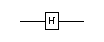
\includegraphics[scale=2]{Figures/circuits/H}};
\end{tikzpicture}
\caption{Clifford+T gates}
\label{fig:clifford}
\end{figure}

\begin{figure}
\vspace*{31mm}
\hspace*{72mm}
\begin{tikzpicture}[transform canvas={scale=0.8}]
  \node[font=\itshape\large] (textgg) {\(\forall g\in\{H,X,Y,Z\}\) cancels itself};
  \node[below=-5mm of textgg] (gg) {
    \begin{tikzpicture}
      \node[inner sep=0pt] (c1) at (0,0) {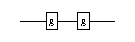
\includegraphics[scale=2]{Figures/circuits/gg}};  
      \node[right=-12mm of c1.east, rectangle, fill=white, minimum size=10mm] (eq) {\(=\)};    
      \node[right=-7mm of eq, inner sep=0pt] (c2) {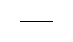
\includegraphics[scale=2]{Figures/circuits/I}};
      \node[right=7mm of c1.west, rectangle,fill=white,minimum size=5mm] {};
      %\node[below right=-1mm and -23mm of eq] (alg) {\small \(g\in\{H,X,Y,Z\}\)};
    \end{tikzpicture}
  };
  \node[above right=28mm and 13mm of textgg, font=\itshape\large] (textCNOT) {CNOT flip};
  \node [below=-5mm of textCNOT] (CNOT) {
    \begin{tikzpicture}
      \node[inner sep=0pt] (c1) at (0,0) {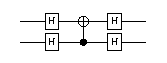
\includegraphics[scale=2]{Figures/circuits/HCNOTH}};       
      \node[right=-13.9mm of c1.east, inner sep=0pt] (c2) {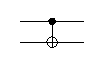
\includegraphics[scale=2]{Figures/circuits/CNOT}};
      \node[right=-12mm of c1.east, rectangle, fill=white, minimum size=10mm] (eq) {\(=\)};  
      \node[right=7mm of c1.west, rectangle,fill=white,minimum width=5mm, minimum height=10mm] {};
      \node[left=7mm of c2.east, rectangle,fill=white,minimum width=5mm, minimum height=10mm] {};
    \end{tikzpicture}
  };
  \node[above left=28mm and 0mm of textgg, font=\itshape\large] (textHXZ) {Rules with \(H\), \(X\), \(Y\) and \(Z\)};
  \node [below left=-5mm and -37mm of textHXZ] (XZ) {
    \begin{tikzpicture}
      \node[inner sep=0pt] (c1) at (0,0) {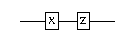
\includegraphics[scale=2]{Figures/circuits/XZ}};       
      \node[below=-3mm of c1] (eq) {\(=\)};  
      \node[below=-3mm of eq, inner sep=0pt] (c2) {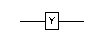
\includegraphics[scale=2]{Figures/circuits/Y}};
      \node[below=-3mm of c2] (eq2) {\(=\)};  
      \node[below=-3mm of eq2, inner sep=0pt] (c3) {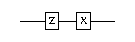
\includegraphics[scale=2]{Figures/circuits/ZX}};
      \node[right=7mm of c1.west, rectangle,fill=white,minimum size=5mm] {};
      \node[left=7mm of c3.east, rectangle,fill=white,minimum size=5mm] {};
      \node[left=7mm of c1.east, rectangle,fill=white,minimum size=5mm] {};
      \node[right=7mm of c3.west, rectangle,fill=white,minimum size=5mm] {};
    \end{tikzpicture}
  };
  \node [below right=-5mm and -37mm of textHXZ] (XH) {
    \begin{tikzpicture}
      \node[inner sep=0pt] (c1) at (0,0) {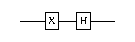
\includegraphics[scale=2]{Figures/circuits/XH}};       
      \node[below=-3mm of c1] (eq) {\(=\)};  
      \node[below=-3mm of eq, inner sep=0pt] (c2) {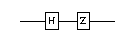
\includegraphics[scale=2]{Figures/circuits/HZ}};
      \node[right=7mm of c1.west, rectangle,fill=white,minimum size=5mm] {};
      \node[left=7mm of c2.east, rectangle,fill=white,minimum size=5mm] {};
      \node[left=7mm of c1.east, rectangle,fill=white,minimum size=5mm] {};
      \node[right=7mm of c2.west, rectangle,fill=white,minimum size=5mm] {};
    \end{tikzpicture}
  };  
  \node[below left=8mm and 7mm of textgg, font=\itshape\large] (textZS) {Rules with \(Z\), \(S\) and \(T\)};
  \node [below left=-5mm and -34mm of textZS] (ZS) {
    \begin{tikzpicture}
      \node[inner sep=0pt] (c1) at (0,0) {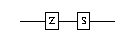
\includegraphics[scale=2]{Figures/circuits/ZS}};       
      \node[below=-3mm of c1] (eq) {\(=\)};  
      \node[below=-3mm of eq, inner sep=0pt] (c2) {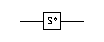
\includegraphics[scale=2]{Figures/circuits/S'}};
      \node[right=7mm of c1.west, rectangle,fill=white,minimum size=5mm] {};
      \node[left=7mm of c1.east, rectangle,fill=white,minimum size=5mm] {};
    \end{tikzpicture}
  };
  \node [below right=-5mm and -34mm of textZS] (ZT) {
    \begin{tikzpicture}
      \node[inner sep=0pt] (c1) at (0,0) {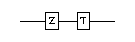
\includegraphics[scale=2]{Figures/circuits/ZT}};       
      \node[below=-3mm of c1] (eq) {\(=\)};  
      \node[below=-3mm of eq, inner sep=0pt] (c2) {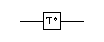
\includegraphics[scale=2]{Figures/circuits/T'}};
      \node[right=7mm of c1.west, rectangle,fill=white,minimum size=5mm] {};
      \node[left=7mm of c1.east, rectangle,fill=white,minimum size=5mm] {};
    \end{tikzpicture}
  };
  \node[below right=8mm and 3mm of textgg, font=\itshape\large] (textXS) {Rules with \(X\), \(S\) and \(T\)};
  \node [below left=-5mm and -34mm of textXS] (XS) {
    \begin{tikzpicture}
      \node[inner sep=0pt] (c1) at (0,0) {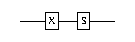
\includegraphics[scale=2]{Figures/circuits/XS}};       
      \node[below=-3mm of c1] (eq) {\(=\)};  
      \node[below=-3mm of eq, inner sep=0pt] (c2) {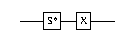
\includegraphics[scale=2]{Figures/circuits/SX}};
      \node[right=7mm of c1.west, rectangle,fill=white,minimum size=5mm] {};
      \node[left=7mm of c2.east, rectangle,fill=white,minimum size=5mm] {};
      \node[left=7mm of c1.east, rectangle,fill=white,minimum size=5mm] {};
      \node[right=7mm of c2.west, rectangle,fill=white,minimum size=5mm] {};
    \end{tikzpicture}
  };
  \node [below right=-5mm and -34mm of textXS] (XT) {
    \begin{tikzpicture}
      \node[inner sep=0pt] (c1) at (0,0) {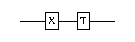
\includegraphics[scale=2]{Figures/circuits/XT}};       
      \node[below=-3mm of c1] (eq) {\(=\)};  
      \node[below=-3mm of eq, inner sep=0pt] (c2) {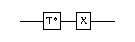
\includegraphics[scale=2]{Figures/circuits/TX}};
      \node[right=7mm of c1.west, rectangle,fill=white,minimum size=5mm] {};
      \node[left=7mm of c2.east, rectangle,fill=white,minimum size=5mm] {};
      \node[left=7mm of c1.east, rectangle,fill=white,minimum size=5mm] {};
      \node[right=7mm of c2.west, rectangle,fill=white,minimum size=5mm] {};
    \end{tikzpicture}
  };
\end{tikzpicture}
\vspace*{35mm}
\caption{Some basic properties of the gates in the Clifford+T set. Here, \(S^*\) and \(T^*\) represent the inverse gates of \(S\) and \(T\), i.e. their conjugate transpose, usually written as \(S^\dag\) and \(T^\dag\).}
\label{fig:props}
\end{figure}

The CNOT gate is particularly interesting. The qubit where the filled dot is (see Figure~\ref{fig:clifford}) acts as the `control', and the qubit with \(\oplus\) acts as the `target'. Whenever the control is \(\ket{0}\), no change is made in either of the qubits; but if it is \(\ket{1}\), an \(X\) gate is applied to the target, flipping the state of the qubit. This works in any superposition, so given an arbitrary two-qubit state \[\ket{c,t} = \alpha\ket{0,0} + \beta\ket{0,1} + \gamma\ket{1,0} + \delta\ket{1,1}\] if the CNOT were to act in \(\ket{c}\) as control and in \(\ket{t}\) as target, the outcome would be: \[CNOT \cdot \ket{c,t} = \alpha\ket{0,0} + \beta\ket{0,1} + \gamma\ket{1,1} + \delta\ket{1,0}\]

\textbf{MBQC model.} The acronym stand for Measurement Based Quantum Computing. Unlike the circuit model, where measurements are done at the very end of the circuit, MBQC carries out computations by means of repeatedly measuring an initially entangled resource. The process can be thought of as sculpting a rock. The rock would be the initial resource, which is a collection of entangled qubits forming certain lattice structure. By measuring some qubits in the lattice -- hitting the rock with a chisel -- we remove some of the excess qubits, changing the overall state in the process. The outcome of measurements is probabilistic so, in order to provide deterministic computation, we must apply corrections on the neighbouring qubits whenever the measurement outcome deviated from the desired result. After multiple iterations of measurements and corrections, we end up with a set of qubits encoding the result. In this model, the input is incorporated into the lattice at the beginning of the process.

In this way, any computation may be performed by applying 1-qubit measurements and 1-qubit correcting gates (controlled by classical signals). The initial resource state contains all the entanglement that is required, which may be prepared experimentally through multi-qubit interactions, such as Ising interactions~\citep{1WQC}, which are within our experimental capabilities. This model deals with the connectivity problem by applying a single operation involving \textit{all} the qubits at the beginning of the process, then only requiring cheap single qubit operations for the rest of the computation. The main drawback of MBQC is the large amount of qubits that are required for even the simplest of operations. The MBQC model was proposed for the first time by \citet{1WQC} under the name of \textit{one-way quantum computer}, which highlights its main difference with the circuit (reversible) approach. 

\textbf{Distributed model.} We may find a balance between the circuit model and MBQC. In it, multiple small quantum processing units (QPUs) would run fragments of the overall circuit. Communication is achieved through a shared entangled resource, reminiscent of the MBQC approach. This model has been discussed in detail in the literature~\citep{DistributedQCHW} and it is at the core of the main project from the Networked Quantum Information Technologies Hub (NQIT)\footnote{A project supported by the UK National Quantum Technology program, aiming to provide scalable quantum computing.}. In \S\ref{DQC_Architecture}, we discuss an abstract distributed quantum architecture in detail.



\section{Programming on quantum computers}

As of today, most quantum programming languages are merely high level circuit descriptors, providing the means to define circuits gate by gate, or build them up from combinations of smaller circuits. All of the well-known languages belong to this category, such as \textit{QCL}~\citep{QCL} (imperative paradigm, and one of the first quantum programming languages ever implemented), \textit{Q\#}~\citep{QLang} (imperative, designed by Microsoft), and \textit{Quipper}~\citep{Quipper} (functional, built on top of Haskell). 

Besides, there are attempts at designing quantum programming languages that are completely hardware agnostic, meaning they aim to describe the computation, rather than a particular circuit that implements it. Examples of these are the different attempts at defining a quantum lambda calculus, for instance the ones by \citet{VanTonder} or \citet{Diaz-Caro}. However, these are not particularly programmer friendly, as they are generally quite verbose.

Most of the literature on quantum algorithms describes them by explicitly giving a circuit that implements the algorithm. Fortunately, there is a constructive procedure, given by the Solovay-Kitaev theorem -- of which \citet{SolovayKitaev} give a good introductory review --, that takes any circuit and a choice of universal gate-set and outputs an equivalent circuit using only those gates. In particular, for the case of the Clifford+T gate set, \citet{OptimalCliffordT} gave an algorithm that outputs the optimal implementation of some quantum operations on this gate set. Hence, programmers do not need to worry about the gates they are using when describing their circuits.

Unfortunately, the fact that algorithms are almost exclusively defined in the circuit model implies that other models of quantum computing are disregarded by a large portion of the community. In order to make other models of computation accessible, we need to provide automated procedures for transforming algorithms from the circuit model to the rest (and vice versa). Work has been done on the transformation from circuit to MBQC and backwards, the latter being the most challenging~\citep{gflow}. However, there is little amount of literature describing how to go from the circuit model to the distributed model. In \S\ref{IntroDistributing} we give an overview of the existent work on that aspect, and identify the gap on the literature we aim to cover in this thesis.

%\begin{mdframed}[backgroundcolor=gray!20,leftmargin=20pt,rightmargin=20pt, innerbottommargin=10pt] 
\begin{remark} \normalfont 
Here are the key concepts to keep in mind while reading the rest of this thesis:
\begin{itemize}
\item Quantum computers provide a computing power well beyond the capabilities of classical computers, which would be exploitable in many areas of science.
\item Small quantum computers are already available. 
\item Scaling up is a challenging problem due to: \textit{decoherence}, which may be overcome by the joint effort of the error-correction, physics and engineering communities; and \textit{connectivity}, which may be solved using distributed architectures.
\item There is practically no programming support for distributed architectures.
\end{itemize}
\end{remark}
%\end{mdframed}